\documentclass[tikz,border=2pt]{standalone}
\usepackage{amsmath}
\usepackage{pgfplots}
\pgfplotsset{compat=1.18}

\begin{document}
% A bounded function stays inside a horizontal strip |f(x)| <= M for every x in the domain.
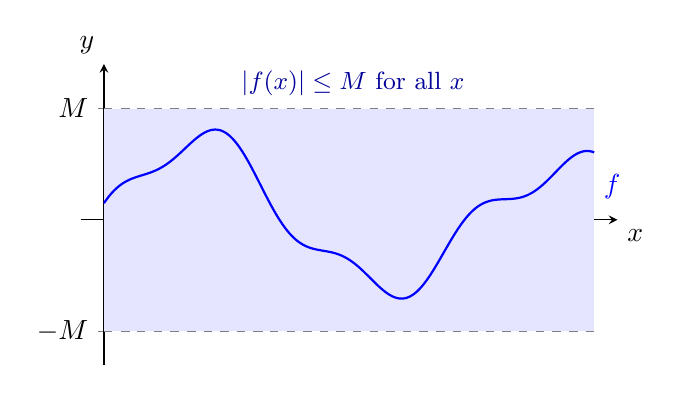
\begin{tikzpicture}
	\begin{axis}[
		axis lines=middle,
		xmin=-0.3, xmax=6.6,
		ymin=-2.6, ymax=2.8,
		xtick=\empty, ytick={-2,2}, yticklabels={$-M$,$M$},
		xlabel={$x$}, ylabel={$y$},
		xlabel style={below right}, ylabel style={above left},
		samples=200, smooth, clip=false,
		width=8.4cm, height=5.4cm
		]
		\fill[blue!10] (axis cs:0,-2) rectangle (axis cs:6.3,2);
		\addplot[gray, dashed, domain=0:6.3] {2};
		\addplot[gray, dashed, domain=0:6.3] {-2};
		\addplot[thick, blue, domain=0:6.3] {1.6*sin(deg(1.3*x))*exp(-0.08*x)+0.3*cos(deg(4*x))};
		\node[blue, anchor=west] at (axis cs:6.3,0.6) {$f$};
		\node[blue!60!black, anchor=south, font=\small] at (axis cs:3.2,2.05) {$|f(x)|\le M$ for all $x$};
	\end{axis}
\end{tikzpicture}
\end{document}
